\documentclass[final]{proposal}
\usepackage[utf8]{vietnam}
\usepackage{placeins}
\usepackage{amsfonts}
\usepackage{textcomp}
\usepackage{dblfloatfix}
\usepackage{lineno}
\usepackage{amssymb}
\usepackage{tabularx,booktabs}
\usepackage{longtable, lipsum}
\usepackage{amsmath}
\usepackage{mathtools}
\usepackage{graphicx}
\usepackage{lscape}
\usepackage{caption}
\usepackage{hyperref}
\usepackage[sorting=nyt]{biblatex}
\usepackage{mathtools}
\usepackage{lipsum}
\usepackage{fancyhdr}
\usepackage{titlesec}
\usepackage{makecell}
\usepackage{listings}
\usepackage{subcaption}
\usepackage{adjustbox}
\usepackage[vietnamese,english]{babel}
\usepackage{multirow}
\usepackage{longtable}
\usepackage{rotating}
\usepackage{chngcntr}
% \usepackage{background}

% Define color and column type
\definecolor{dkgreen}{rgb}{0,0.6,0}
\definecolor{gray}{rgb}{0.5,0.5,0.5}
\definecolor{mauve}{rgb}{0.58,0,0.82}
\newcolumntype{C}[1]{>{\centering\arraybackslash}m{#1}}

% Config reference source file
\addbibresource{references/references.bib}

% Config figure path
\graphicspath{ {./graphics} }

% Config for math in quantum computin
\DeclarePairedDelimiter\bra{\langle}{\rvert}
\DeclarePairedDelimiter\ket{\lvert}{\rangle}
\DeclarePairedDelimiterX\braket[2]{\langle}{\rangle}{#1 \delimsize\vert#2}

% Config listings 
\lstset{
  frame=tb,
  aboveskip=3mm,
  belowskip=3mm,
  showstringspaces=false,
  columns=fullflexible,
  basicstyle={\small\ttfamily},
  numbers=left,
  numberstyle=\tiny\color{gray},
  keywordstyle=\color{blue},
  commentstyle=\color{dkgreen},
  stringstyle=\color{mauve},
  breaklines=true,
  postbreak=\mbox{\textcolor{red}{$\hookrightarrow$}\space},
  tabsize=3
}


% Config information thesis
% =========== Thay đổi thông tin tại phần này ===========
\upperuniname{ĐẠI HỌC QUỐC GIA THÀNH PHỐ HỒ CHÍ MINH}
\uniname{TRƯỜNG ĐẠI HỌC CÔNG NGHỆ THÔNG TIN}
\title{MAGIC: Detecting Advanced Persistent Threats via Masked Graph Representation Learning}
% \titleen{MAGIC: Detecting Advanced Persistent Threats via Masked Graph Representation Learning}
\supervisorname{TS. LÊ KIM HÙNG }
\stuname{230202002 - Tô Thị Mỹ Âu\\220202022 - Nguyễn Hồng Sơn \\230202006 - Ngô Thái Hưng  }
\proposaltype{Máy học trong bảo mật mạng và hệ thống}
\reportplace{TP. HỒ CHÍ MINH, NĂM }
% =========== Hết phần thay đổi thông tin ===========
% \backgroundsetup{contents=Templates,placement=center,color=pink}


% Begin thesis
\begin{document}


\headerbox
\vnproposalheader
\proposalname
\frontmatter
\tableofcontents
% Begin main thesis, start page numbering
\mainmatter

\counterwithin{equation}{section}
\counterwithin{table}{section}
\counterwithin{figure}{section}
\setcounter{secnumdepth}{3}



% \input{sections/summary.tex}
\pagestyle{fancy}
\fancyhf{}
\fancyfoot[C]{\thepage}
\if @twoside
  \fancyhead[EL,OR]{\bfseries\nouppercase\rightmark}
\else
  \fancyhead[R]{\bfseries\nouppercase\rightmark}
\fi


\section{Tóm tắt bài báo}

MAGIC là một phương pháp học có giám sát để phát hiện các cuộc tấn công APTs bằng cách sử dụng phương pháp học masked graph representation. Nó cải thiện một số phương pháp trước đó bằng cách trích xuất efficient deep feature và structure abstraction on provenance graphs.

MAGIC có khả năng phát hiện multi-granularity, handle concept drift with a model adaption mechanism và có khả năng mở rộng. Nó sử dụng phương pháp phát hiện ngoại lệ để xác định hành vi bất thường.

MAGIC được đánh giá dựa trên 3 dataset, cho kết quả phát hiện với chỉ số precision và recall cao, chi phí thấp và nhanh hơn nhiều so với các phương pháp hiện tại

Các kết quả của bài báo là một công trình được phát hành dưới dạng opensource, với tiềm năng phát triển nhiều trong lương lai.

\section{Experiments}
%------------------------------------------------

% \begin{frame}{Single images}
%    \begin{figure}[h]
%        \centering
%        
\includegraphics[width=0.7\textwidth]{img/logo_v2.png}
%        \caption{Slide with single images}
%        \label{fig:sing_image}
%    \end{figure}
% \end{frame}

% %------------------------------------------------

% \begin{frame}{Single image with itemize}
%      Lorem ipsum dolor sit amet, consectetur adipiscing elit:
%     \begin{enumerate}
%         \item Lorem ipsum dolor sit amet.
%         \item Lorem ipsum dolor sit amet.
%     \end{enumerate}
    
%    \begin{figure}[h]
%        \centering
%        
\includegraphics[width=0.7\textwidth]{img/logo_v2.png}
%        \caption{Slide with single images}
%        \label{fig:sing_image}
%    \end{figure}
% \end{frame}

%------------------------------------------------
\begin{frame}{Methodology}

\begin{columns}

\column{0.3\textwidth}
 \footnotesize
    \begin{thebibliography}{99}
        \bibitem{autorlivro} Zhang, Yinghua, et al. "Two sides of the same coin: White-box and black-box attacks for transfer learning." Proceedings of the 26th ACM SIGKDD international conference on knowledge discovery \& data mining. 2020.

    \end{thebibliography}

\column{0.7\textwidth}
    \begin{figure}
        \begin{subfigure}{0.9\textwidth}
            \centering
            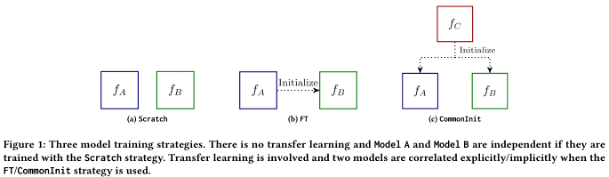
\includegraphics[scale=0.55]{img/exper-1.png}
     
            \label{fig:sub-figure-url-1}
        \end{subfigure} \\
        \begin{subfigure}{0.9\textwidth}
            \centering
            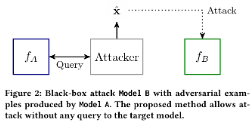
\includegraphics[scale=0.55]{img/exper-2.png}
    
            \label{fig:sub-figure-url-2}
        \end{subfigure}
        \label{fig:example-subfigure}
    \end{figure}
    \begin{itemize}
        \item Datasets: MNIST (M), USPS (U), SVHN (S), SynDigits (Syn), CIFAR10, STL10, ImageNet32
    \end{itemize}
\end{columns}

\end{frame}

%------------------------------------------------
\begin{frame}{White-box Attack Experiment}
\begin{columns}[T]
    \column{0.4\textwidth}
        \begin{itemize}
            \item \textbf{Goal}: Assess robustness to FGSM attacks.
            \item \textbf{Method}: Compare Scratch vs. Fine-tuning models under various noise levels.
            \item \textbf{Result}:
            \begin{itemize}
                \item Fine-tuning significantly improves accuracy and robustness.
                \item Example: Accuracy increases from 50.86\% -> 84.96\% at $\epsilon = 0.125$.
            \end{itemize}
            % \item \textbf{Conclusion}: Fine-tuning enhances both performance and security.
        \end{itemize}

    \column{0.6\textwidth}
       \begin{figure}[h]
           \centering
           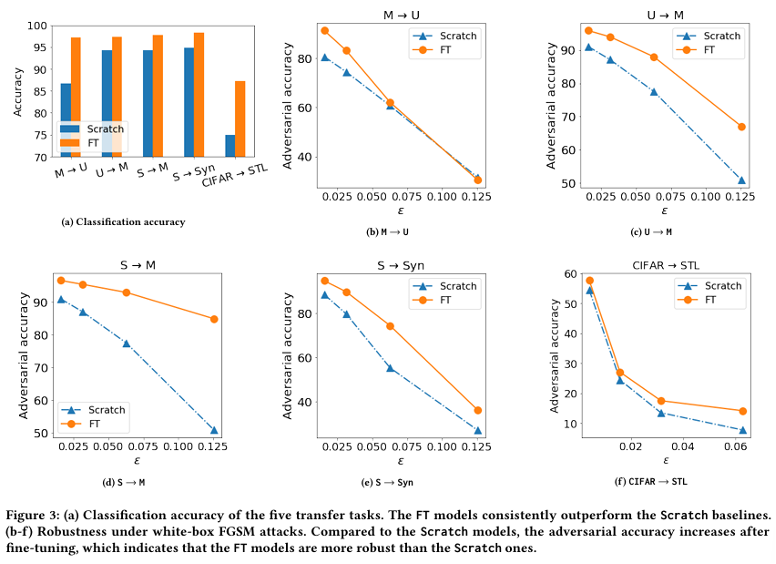
\includegraphics[scale=0.7]{img/white-box.png}
           \label{fig:what-is}
       \end{figure}
    \end{columns}
\end{frame}
%------------------------------------------------
\begin{frame}{Black-box Attack Experiment}
\begin{columns}[T]
    \column{0.6\textwidth}
       \begin{figure}[h]
           \centering
           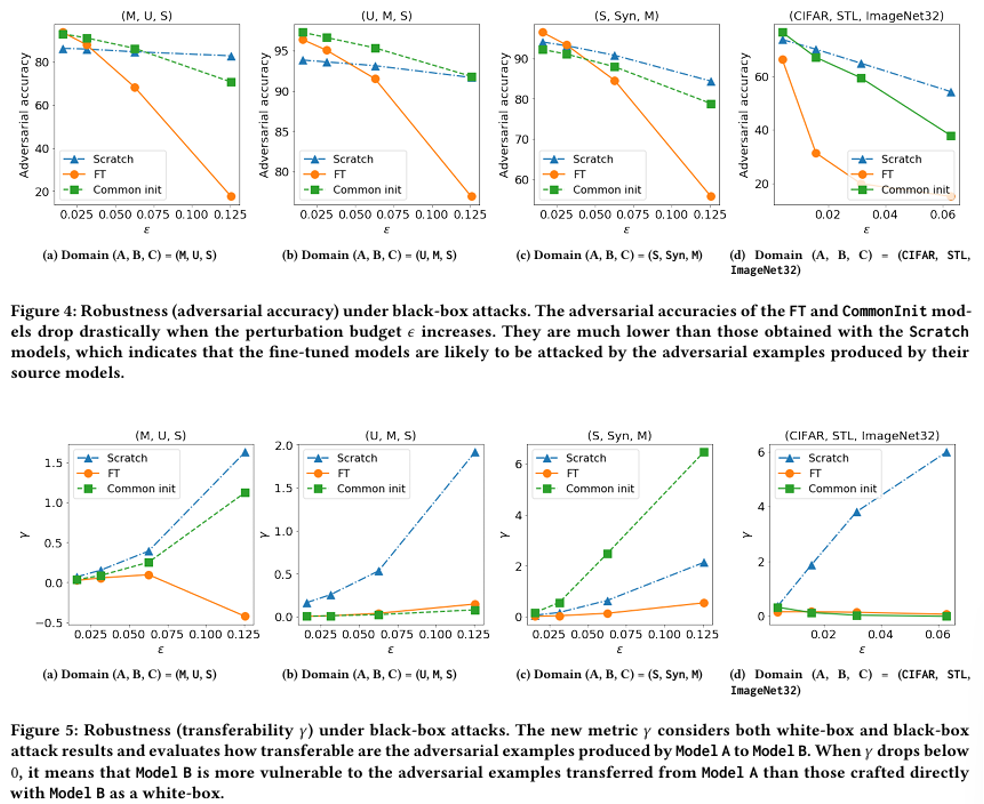
\includegraphics[scale=0.5]{img/black-box.png}
           \label{fig:black-box}
       \end{figure}
    \column{0.4\textwidth}
        \begin{itemize}
            \item \textbf{Goal}: Evaluate transferability of adversarial examples.
            \item \textbf{Method}: Attack model B using adversarial examples from model A.
            \item \textbf{Result}:
            \begin{itemize}
                \item Fine-tuned models are more vulnerable to transferred attacks.
                \item Example: Accuracy drops from 87.43\% -> 65.32\% (FGSM).
            \end{itemize}
            % \item \textbf{Conclusion}: Fine-tuning improves performance but increases attack susceptibility.
        \end{itemize}
\end{columns}
\end{frame}

%------------------------------------------------


\newpage
\printbibliography[heading=bibintoc, title = {Tài liệu tham khảo}]
\end{document}